\section{Validation de la simulation}
La simulation d'une hiérarchie de caches étant un problème relativement compliqué, il convient de valider le fonctionnement du logiciel par différentes études des statistiques produites.

\subsection{Tests unitaires}

Quelques tests unitaires basiques ont été mis en place afin de valider les bases du logiciel. Ces tests portent notamment sur la création du fichier décrivant l'architecture à partir d'un fichier xml généré par hwloc. Ils permettent également de s'assurer de la justesse des politiques de cohérence et de remplacement pour un petit ensemble de données. En vérifiant le remplissage et les évictions de données, de même que les flags utiles aux protocoles de cohérence, quelques problèmes sont déjà levés. \\

Par ailleurs, même si cela ne constitue pas des tests unitaires, des vérifications sont réalisées au sein du code, afin de valider le caractère inclusif ou exclusif des caches. Des messages d'erreur sont renvoyées quand les propriétés des caches ne sont plus respectées, ce qui notamment permis de déceler beaucoup de problèmes durant la phase de développement du simulateur.

\subsection{Validation comparative}

Les tests unitaires sont assez limités au sens où la validation complète du logiciel impose d'étudier l'ensemble des cas pouvant se produire sur un ensemble assez conséquent de données. Connaître précisement les résultats après $n$ opérations en déroulant soi-même l'execution de ces instructions est délicat. Il a donc fallut se tourner vers d'autres moyens de vérification. \\

Dans un premier temps, le logiciel PAPI (Performance Application Programming Interface), permettant d'utiliser les compteurs hardware d'une machine données, a été utilisé. Ce logiciel permet d'exploiter les compteurs hardware natifs présents dans les processeurs actuels. Nous avons donc utilisé ces compteurs, afin de comparer nos résultats avec les résultats obtenus sur différentes architectures. \\

Le problème posé ici est que les caches ne constituent pas l'unique solution par rapport au problème de l'accès à la mémoire principale. En effet, un autre phénomène, le \emph{prefetching}, est mis en place, et il permet notamment d'éviter les \emph{compulsory misses}, c'est-à-dire les \emph{misses} qui interviennent au moment où l'on charge les données dans les caches. Par exemple, lors du chargement d'un tableau, le \emph{prefetching} permet de détecter qu'on est en train de charger progressivement une zone mémoire contigue, et précharge donc les données à un emplacement proche des caches. L'accès n'est alors plus compté comme un \emph{miss}. \\

La validation comparative s'est donc révelée être un échec, les écarts entre notre simulation et les compteurs hardware étant théoriquement trop conséquents pour conclure objectivement quant aux statistiques obtenues. Par ailleurs, l'étude d'autres simulateurs de caches s'est également révelée infructueuse. Par exemple, un module du logiciel \textsf{Valgrind}, nommé \textsf{Cachegrind}, permet de donner les pourcentages de \emph{hits} et de \emph{misses} pour l'execution d'un programme. Malheureusement, leur émulation ne simule pas un comportement multi-threadés, et il a encore été impossible de conclure.
 
\subsection{Benchmarks}
La validation du simulateur a donc été possible en étudiant des codes connus pour être plus ou moins bons d'un point de vue des caches. L'étude porte sur une architecture de type \textsf{Intel} i3, i5 ou i7. Il y a $4$ caches L1, $2$ caches L2 exclusifs et $1$ L3 inclusif. La fonction ``par'' réalise des écritures sur un tableau en le partageant correctement entre les différents c{\oe}urs. La fonction ``falsesharing'' réalise une opération semblable, mais des lignes de cache sont utilisées simultanément par plusieurs c{\oe}urs. Avec la fonction ``broadcast'', tous les threads accèdent aux données du premier et avec la fonction ``pipeline'', il y a également des échanges entre les caches. \\

Il faut noter que l'entrelacement choisi est d'effectuer une instruction par c{\oe}ur avant de passer au c{\oe}ur suivant. Pour plus d'informations sur l'architecture étudiée (taille, associativité des caches \dots) voir la partie \emph{bench} dans le code source. Par ailleurs, seules les instructions opérant en dehors de la pile sont prises en compte. En effet, étudier les statistiques relatives à la pile est peu intéressant, car il y a beaucoup de \emph{misses}, alors que les instructions relatives aux données (dans le tas par exemple) sont source de beaucoup plus de disparités. Les graphiques suivants résument les statistiques basiques pour chaque niveau de cache, en faisant une moyenne lorsqu'il y a plusieurs caches pour un seul niveau.\\

\begin{figure}[H]
   \begin{minipage}[l]{.46\textwidth}
     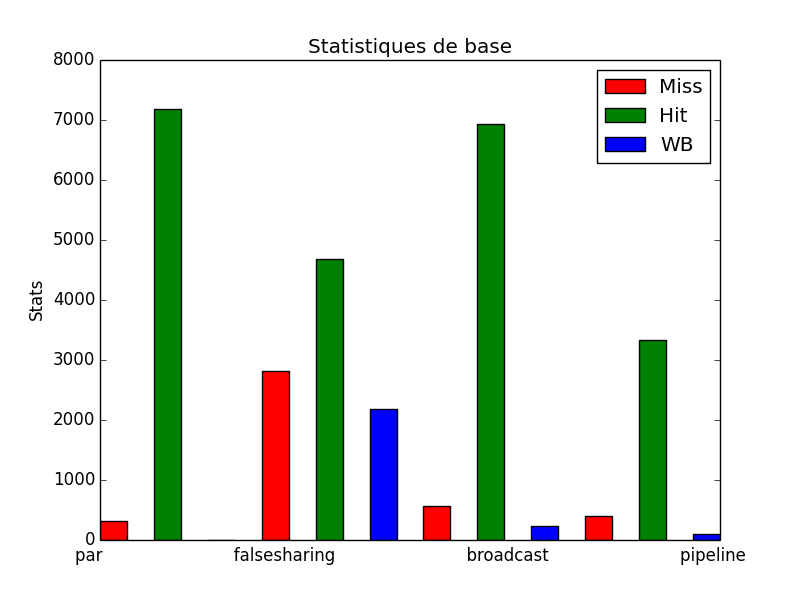
\includegraphics[scale=0.35]{images/stats_L1.png}
     \caption{\label{img:inclusifs} Statistiques pour les L1 avec des problèmes connus}
   \end{minipage} \hfill
   \begin{minipage}[r]{.46\textwidth}
     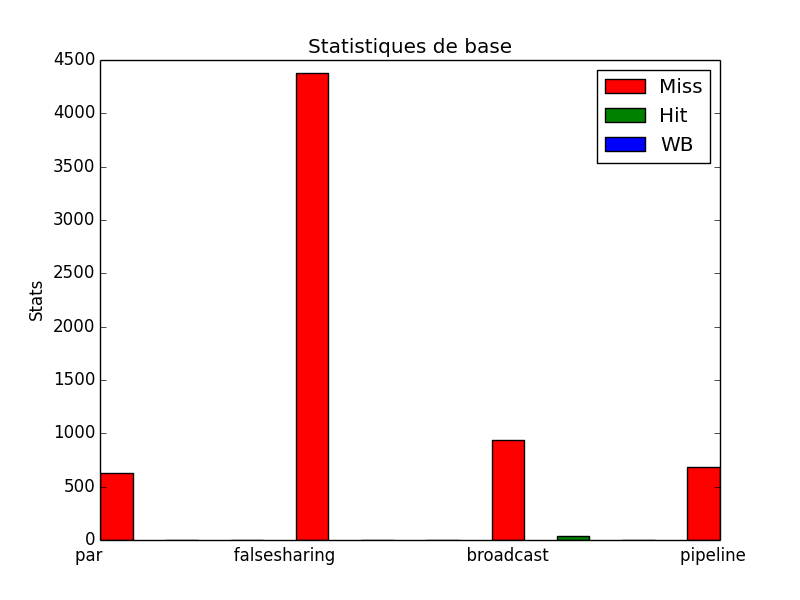
\includegraphics[scale=0.35]{images/stats_L2.png}
     \caption{\label{img:inclusifs} Statistiques pour les L2 avec des problèmes connus}
   \end{minipage}
\end{figure}

\begin{figure}[H]
\begin{center}
   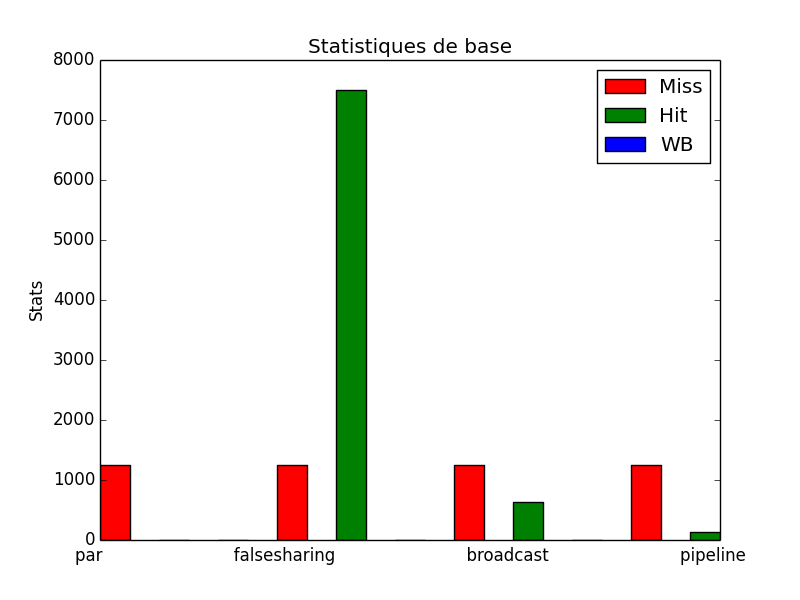
\includegraphics[scale=0.35]{images/stats_L3.png}
   \caption{\label{img:inclusifs} Statistiques pour les L3 avec des problèmes connus}
\end{center}
\end{figure}

Ces trois premiers graphiques permettent de valider le comportement global du simulateur. Dans le cas où les données sont correctement partagées, les statistiques sont bien meilleures. Par ailleurs, les seules interactions avec le cache L3 pour la fonction ``par'' sont celles qui correspondent aux \emph{compulsory misses}, alors que pour la fonction ``falsesharing'', d'autres interactions sont nécessaires à cause des problèmes de cohérence dans les plus bas niveaux. \\

Une autre étude permet de valider en partie le fonctionnement du \emph{snooping}. Avec cette technique, les interactions entre les L1 sont privilégiées et évitent d'accèder aux plus hauts niveaux. On retrouve cette idée sur les deux graphiques qui suivent où, si les statistiques pour les L1 sont semblables, la manière de récupérer les données avec le snooping nécessite moins de requêtes aux niveaux supérieurs. On note un gain de vitesse d'environ 50\% dû au temps gagné sur les \emph{misses} qui prennent environ 10 fois plus de temps à traiter que les \emph{hits}.\\

\begin{figure}[H]
   \begin{minipage}[l]{.46\textwidth}
     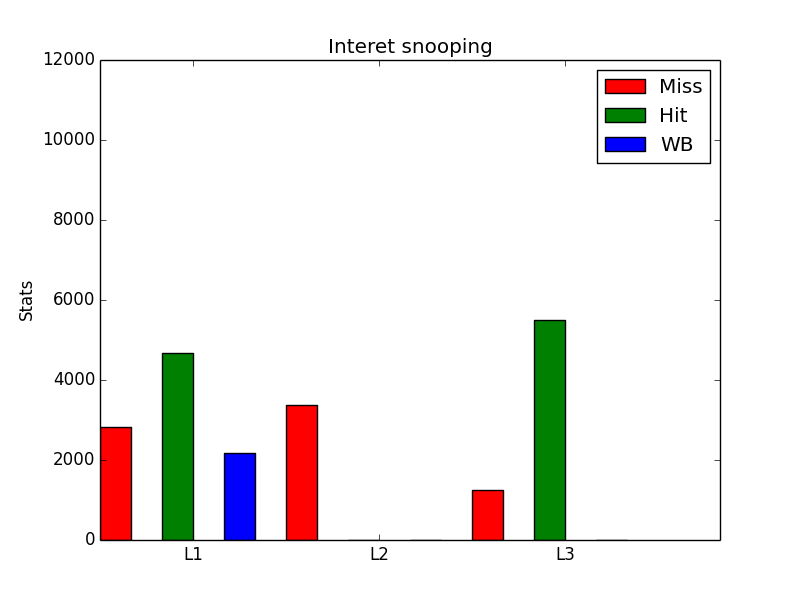
\includegraphics[scale=0.35]{images/stats_falsesharing_snooping.png}
     \caption{\label{img:inclusifs} Statistiques de la fonction falsesharing avec du snooping}
   \end{minipage} \hfill
   \begin{minipage}[r]{.46\textwidth}
     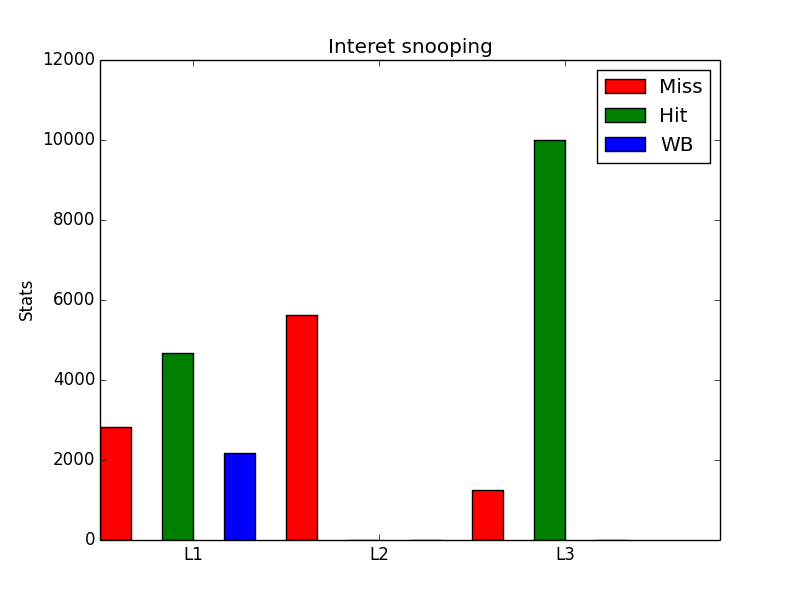
\includegraphics[scale=0.35]{images/stats_falsesharing_no_snooping.png}
     \caption{\label{img:inclusifs} Statistiques de la fonction falsesharing sans snooping}
   \end{minipage}
\end{figure}

La dernière fonctionnalité importante du simulateur est l'ajout des \emph{directory manager}, qui permettent de gérer plus subtilement les évictions et de rechercher les données dans un cache de dernier niveau non inclusif. Dans les graphiques suivant, on peut observer l'apport des \emph{directory manager}. Les différences sont certes minimes, mais permettent parfois de réelles optimisations. 

\begin{figure}[H]
   \begin{minipage}[l]{.46\textwidth}
     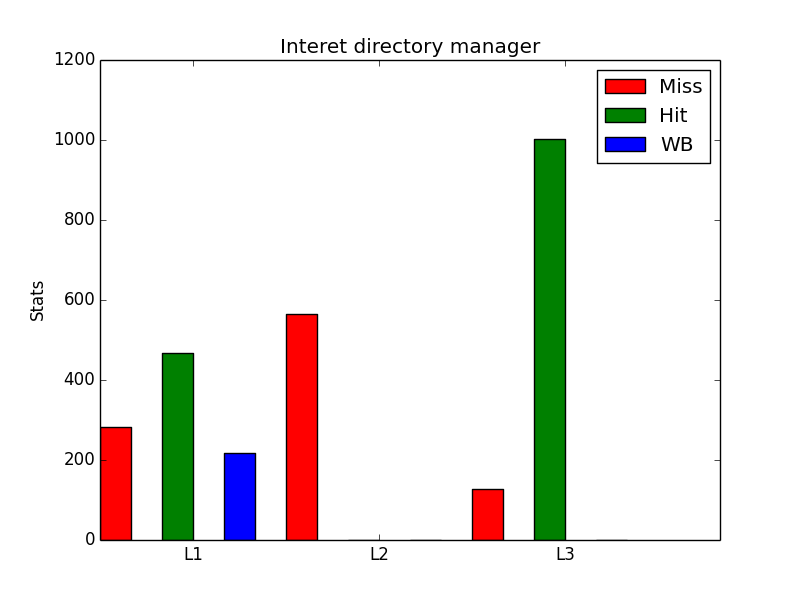
\includegraphics[scale=0.35]{images/stats_falsesharing_directory.png}
     \caption{\label{img:inclusifs} Statistiques de la fonction falsesharing avec des directory manager}
   \end{minipage} \hfill
   \begin{minipage}[r]{.46\textwidth}
     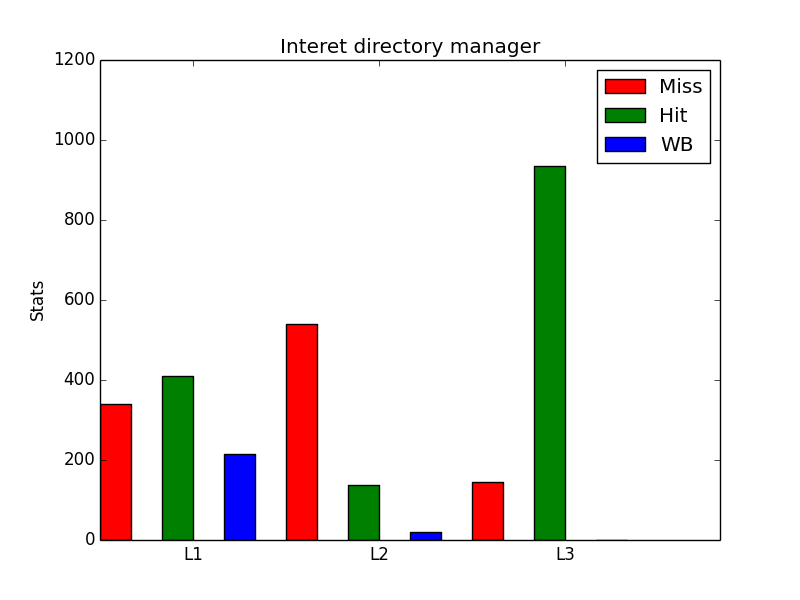
\includegraphics[scale=0.35]{images/stats_falsesharing_no_directory.png}
     \caption{\label{img:inclusifs} Statistiques de la fonction falsesharing sans directory manager}
   \end{minipage}
\end{figure}

Pour les politiques de cohérence, MSI et MESI ont été testé. Sur un exemple basique ou les c{\oe}urs partagent correctement les données entre eux, et où un tableau est lu avant d'être modifié, les résultats attendus sont corrects. En effet, dans le cas de MSI il y a deux fois plus de \emph{broadcast} nécessaires à la gestion de la cohérence que dans le cas de MESI. On voit bien l'apport de l'état E qui permet de modifier une donnée sans informer les autres caches du même niveau, étant donné que la donnée est connue pour être exclusive au cache étudié. \\

Par ailleurs, une petite étude afin de prouver que les performances du logiciel sont bien linéaire en fonction du temps est présentée figure \ref{img:inclusifs}. \\

\begin{figure}[H]
\begin{center}
   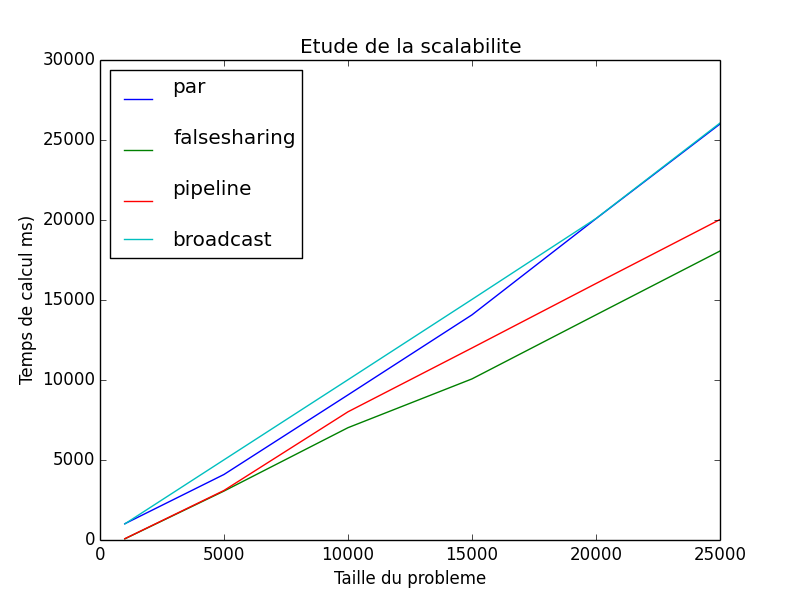
\includegraphics[scale=0.35]{images/scalability.png}
   \caption{\label{img:inclusifs} Etude de la scalabilite du programme}
\end{center}
\end{figure}
